\chapter{Estratégias de otimização}
\label{estrategias-otimizacao}

Nas próximas seções são detalhadas algumas das estruturas e técnicas utilizadas pelos \glspl{dba} quando se deseja obter um melhor desempenho na execução das consultas em bancos de dados relacionais. Na seção \ref{indices} é detalhado o assunto de indexação, mencionando os vários tipos de índices existentes e como são utilizados. A seção \ref{outras-otimizacoes} descreve brevemente outras abordagens existentes para otimização de bancos de dados, como particionamento, visões materializadas e agrupamento de dados.


\section{Índices}
\label{indices}

Um índice é uma estrutura de dados auxiliar utilizada pelo \gls{sgbd} durante a execução de uma consulta para encontrar os dados mais rapidamente \cite[p. 53]{Lightstone:2007}. O uso de índices como forma de localizar dados específicos em um banco de dados é uma das formas mais comuns de otimização e também a que apresenta o melhor resultado quando os índices corretos são selecionados \cite{Petraki:2015}. De forma geral, os índices podem ser classificados em simples ou compostos, primários ou secundários e únicos ou não-únicos.

Os índices simples são formados por apenas um atributo da tabela. Dessa forma, a chave do índice é o valor do atributo indexado, e o índice informa a localização de um ou mais registros da tabela que possuem o mesmo valor da chave para esse atributo. Os índices compostos são criados para múltiplos atributos de uma mesma tabela. A chave do índice, nesse caso, é formada pela concatenação dos valores dos atributos indexados, e indica a localização de registros que possuam os mesmos valores concatenados da chave para os mesmos atributos. Os índices compostos apresentam um desempenho melhor do que o uso de índices simples quando os dados são filtrados por mais de um atributo presente no índice, porém sua utilização é restrita apenas às consultas que se encaixam em alguns critérios \cite[p. 21]{Lightstone:2007}. A ordem dos atributos no índice é importante, uma vez que a chave é formada pela concatenação dos valores, as consultas devem incluir os atributos que estão no começo da chave para utilizar o índice.

Os índices primários definem a organização principal dos dados na tabela. A chave desse tipo de índice, também conhecida como chave primária, deve ser um valor único para cada registro. Esse é um dos índices mais importantes em uma banco de dados, pois a maioria das junções entre tabelas é feita através da chave primária \cite[p. 56--57]{Lightstone:2007}. Cada tabela pode possuir um único índice primário, e todos os outros índices da tabela são chamados de secundários.

Índices únicos são formados por atributos cujos valores não podem ser repetidos em toda a tabela. Todos os índices primários devem ser índices únicos, mas índices secundários também podem ser definidos como tal. Cada entrada em um índice único identifica exclusivamente um registro na tabela, enquanto que em índices não-únicos para cada valor da chave podem existir vários identificadores de linhas na tabela.

Os \glspl{sgbd} relacionais oferecem diferentes estruturas para definição dos índices, sendo as principais e mais utilizadas: \emph{B+tree}, \emph{hash} e \emph{bitmap}. Estas estruturas definem como os dados do índice são organizados em disco e acessados posteriormente na etapa de execução da consulta.

Os índices \emph{B+tree} utilizam uma estrutura de árvore com ponteiros para blocos de dados. O tamanho da árvore varia de acordo com a quantidade de valores distintos existentes para os atributos que compõem o índice. Os nós intermediários da árvore possuem os valores dos atributos ordenados e ponteiros para sub-árvores de busca. Esses valores são utilizados para identificar qual sub-árvore contém a chave pesquisada, reduzindo o espaço de busca e possibilitando encontrar os nós folha de forma eficiente, com poucas operações de entrada/saída de dados.

Os nós folha dos índices \emph{B+tree} possuem as informações realmente importantes: a chave, que são os valores dos atributos que compõem o índice, um identificador de um ou mais registros da tabela que possuem o valor da chave, a partir do qual o \gls{sgbd} pode localizar precisamente a linha indicada, e um ponteiro para o próximo nó folha da árvore, que agiliza buscas por intervalos de valores, acessando diretamente os nós folha sem caminhar pela árvore.

O desempenho desse tipo de índice depende diretamente de sua seletividade, como mostra a figura \ref{fig:btree-index-vs-table-scan}. O tempo necessário para o acesso sequencial à tabela é constante, enquanto que o tempo para leitura dos dados utilizando o índice cresce à medida que mais registros são retornados pela consulta.

\begin{figure}[ht]
  \centering
  \caption{Tempo de acesso ao disco utilizando índice \emph{B+tree} vs. acesso sequencial.}
  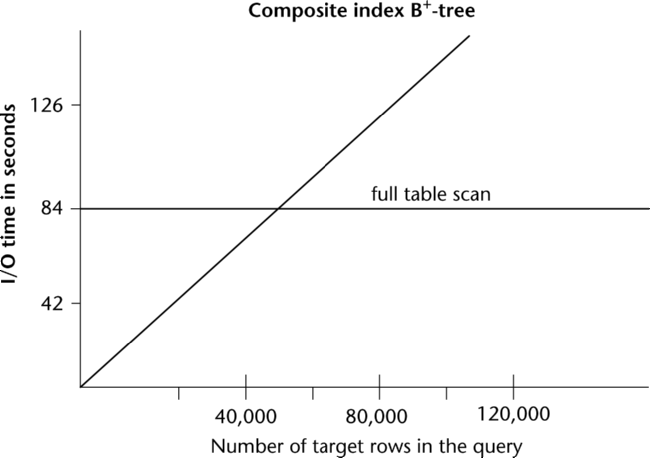
\includegraphics[width=.7\textwidth]{btree-index-vs-table-scan.png}
  \fonte{\citeonline{Lightstone:2007}}
  \label{fig:btree-index-vs-table-scan}
\end{figure}

Os índices do tipo \emph{bitmap} são utilizados para atributos com baixa seletividade, ou seja, com poucos valores diferentes. Cada possível combinação de valores para os atributos do índice possui um vetor de \emph{bits} e cada registro na tabela é representado por um \emph{bit} nesse vetor, sendo que o \emph{bit} é ativado se o registro possui o valor que o respectivo vetor representa. Esse tipo de índice oferece um bom desempenho nas consultas por serem utilizadas operações binárias (E, OU, NÃO) entre os vetores de bits para identificar os registros que possuem uma determinada combinação de valores dos atributos indexados, porém não é facilmente expansível para novos registros e valores de atributos como os índices \emph{B+tree} \cite[p. 27]{Lightstone:2007}.

Índices do tipo \emph{hash} são geralmente utilizados quando os dados de uma tabela não são armazenados em disco de forma ordenada. É utilizada uma função para calcular uma localização em disco a partir do valor da chave, a qual geralmente é criada com atributos que possuem valores únicos. A localização retornada pela função de \emph{hash} identifica o endereço de um bloco inicial, e é utilizado durante as operações de atualização e consulta de dados. Este tipo de índice é recomendado para consultas que acessam um único registro da tabela buscando pelo valor da chave. Entretanto, os índices do tipo \emph{B+tree} oferecem um desempenho equivalente, e, portanto, os índices \emph{hash} são suportados em poucos \glspl{sgbd} \cite[p. 56]{Lightstone:2007}.





\section{Outras otimizações}
\label{outras-otimizacoes}

Além do uso de índices, os \glspl{sgbd} relacionais também oferecem outras estruturas que podem ser utilizadas na definição do modelo físico do banco de dados com o objetivo de reduzir o tempo necessário para acessar os dados. Algumas dessas funcionalidades são o particionamento, as visões materializadas e o agrupamento multidimensional, entre outras menos comuns.

O \textbf{particionamento} é uma técnica de otimização que consiste em dividir grandes volumes de dados em tabelas menores. Existem dois principais métodos para implementar o particionamento: horizontal e vertical. No particionamento horizontal, a estrutura da tabela permanece inalterada, mas o registros são armazenados em arquivos de dados separados. Essa divisão dos dados é feita a partir de algum critério definido previamente pelo \gls{dba}. Nesse tipo de particionamento, os dados são manipulados pelo \gls{sgbd} como se estivessem em tabelas diferentes, com um número menor de registros por tabela, mas para a aplicação que acessa o banco de dados eles continuam sendo apresentados como uma tabela única.

Outra forma de particionamento é o vertical, onde alguns atributos menos utilizados de uma tabela são movidos para outra e apenas uma relação entre os registros é mantida. Assim, o tamanho de cada registro da tabela principal é reduzido, permitindo que o \gls{sgbd} possa carregar mais registros para a memória simultaneamente.

As visões são uma técnica utilizada em bancos de dados para armazenar a definição de uma consulta e permitir que os dados dessa visão sejam acessados posteriormente sem a necessidade de saber como a consulta original foi escrita. As \textbf{visões materializadas} incrementam essa funcionalidade, armazenando o resultado da execução da consulta que forma a visão para que este seja utilizado em consultas subsequentes. Portanto, essa estratégia é útil quando uma determinada visão é acessada frequentemente e não é necessário que o resultado da consulta seja atualizado em todos os acessos.

O agrupamento (\emph{clustering}) simples permite organizar os dados de uma tabela, armazenando os registros que possuem valores de atributos iguais no mesmo bloco em disco. A técnica de \textbf{agrupamento multidimensional} -- \gls{mdc} -- estende o agrupamento simples, permitindo que dentro de um bloco os dados sejam novamente agrupados pelo do valor de outro atributo. Dessa forma, ao executar uma consulta que filtra por um ou mais atributos que fazer parte do agrupamento definido para a tabela, o \gls{sgbd} pode acessar diretamente o bloco no disco que contém as informações desejadas.
